\documentclass[twocolumn]{article}

\usepackage{graphicx}
\usepackage[a4paper, margin=0.5in]{geometry}
\usepackage{amsmath}

\begin{document}

\section*{Equations}
\pagestyle{empty}

\begin{enumerate}
    \item $P = \frac{dW}{dt} = IV$
    \item $I = \frac{dq}{dt}$
    \item $V = \frac{W}{q}$
    \item $R = \frac{\rho L}{A}$
    \item Ohm's Law: $V=IR$
    \item Coulomb's Law: $\vec{F} = \frac{1}{4\pi \epsilon_0}\frac{q_1 q_2}{r^2}\hat{r}$
    \item Kirchhoff's Loop Law: $\sum V_i = 0$ (around a closed loop)
    \item Kirchhoff's Current Law: $\sum I_i = 0$ (going into a node)
    \item Conductance: $G = \frac{1}{R}$
    \item Equivalent resistance: $R_{eq} = \frac{V_{test}}{I_{test}}$
    \item Series capacitance: $\frac{1}{C_{total}} = \frac{1}{C_1} + \frac{1}{C_2} + \dots$
    \item Parallel capacitance: $C_{total} = C_1 + C_2 + \dots$
    \item Series inductor: $L_{total} = L_1+L_2+\dots$
    \item Parallel inductor: $\frac{1}{L_{total}} = \frac{1}{L_1} + \frac{1}{L_1} + \dots$
    \item $I_{cap} = C \frac{dV}{dt}$
    \item $V_{ind} = L \frac{dI}{dt}$
    \item Energy stored in capacitor: $\frac{1}{2}CV^2$
    \item Energy stored in inductor: $\frac{1}{2}LI^2$
    \item Voltage in RC circuit: 
    \[v_c(\infty) +\left(v_c(t_0) - v_c(\infty)\right)e^{(\frac{-1}{RC})(t - t_0)}\]
    \item Current in RL circuit: 
    \[I_L(\infty) +\left(I_L(t_0) - I_L(\infty)\right)e^{(\frac{-R}{L})(t - t_0)}\]
    \item Impedance of a capacitor: $\frac{-j}{\omega C}$
    \item Impedance of an inductor: $j \omega L$
    \item Equivalent impedance for impedances in series: 
    \[Z_{eq} = \sum_{i}^{n} Z_i\]
    \item Equivalent impedance for impedances in parallel: 
    \[\frac{1}{Z_{eq}} = \sum_{i}^{n} \frac{1}{Z_i}\]
    \item RMS value of signal: $S_{rms} = \sqrt{\frac{1}{T}\int_{t_0}^{t_0+T} s^2(t) dt}$
    \item Maximum power extracted in DC circuits: $\frac{V{th}^2}{4R_{th}}$
    \item Maximum power extracted in AC circuits: $\frac{|\tilde{V}_{th}|^2}{8R_{th}}$
    \item Average power: $P_{avg} = \frac{V_m I_m}{2}\cos{(\theta_v - \theta_i)}$
    \item Reactive power: $V_{ar} = Im(\frac{1}{2}\tilde{V}\tilde{I}^*)$
    \item Apparent power: $P_{app} = \frac{|V_{rms}|^2}{|z|}$
    \item Coupling coefficient in coupled circuit: $k = \frac{L_{12}}{\sqrt{L_1 L_2}}$
    \item Voltage in magnetically coupled coils: 
    \begin{align*}
        v_{1}(t) &= L_1 \frac{di_1(t)}{dt} + L_{12}\frac{di_2(t)}{dt} \\
        v_{2}(t) &= L_1 \frac{di_2(t)}{dt} + L_{12}\frac{di_1(t)}{dt} 
    \end{align*}
    \item Voltage in ideal transformer: 
    \begin{align*}
        \frac{v_2(t)}{v_1(t)} &= \frac{N_2}{N_1} \\
        \frac{i_2(t)}{i_1(t)} &= -\frac{N_1}{N_2}   
    \end{align*}
    \item Terminated transformer circuit equations: 
    \begin{align*}
        \tilde{V}_1 &= \frac{\tilde{V}_2}{n} \\
        \tilde{I}_{out} &= \frac{\tilde{I}_{in}}{n} \\
        \tilde{V}_{in} &= Z_{in}\tilde{I}_{in} + \tilde{V}_1 \\
        \tilde{V}_2 &= Z_{out}\tilde{I}_{out} \\
        \tilde{V}_2 &= Z_{out}\frac{\tilde{I}_{in}}{n} \\
        \frac{\tilde{V}_{in}}{\tilde{I}_{in}} &= Z_{in} + \frac{Z_{out}}{n^2}
    \end{align*}
    \item Energy stored in magnetically coupled circuit: 
    \[E = \frac{1}{2}L_1i_1^2 + \frac{1}{2}L_2i_2^2 + L_{12}i_1i_2\]
    \item Equilibrium in pn junction: $pn = n_i^2$
    \item Current in pn junction: 
    \begin{align*}
        J_N &= q\mu_n n E_x + qD_n \frac{dn}{dx} \\
        J_P &= -qD_p \frac{dp}{dx} + q\mu_p p E_x
    \end{align*}
    \item Width of depletion region: 
    \[W = \left[\frac{2\epsilon_r \epsilon_0}{q} \left(\frac{N_A + N_D}{N_A N_D}\right) V_{bi}\right]^{1/2}\]
    \item Built-in potential: $V_{bi} = \frac{kT}{q}\ln{\left(\frac{N_AN_D}{n_i^2}\right)}$
    \item Current through an ideal diode: $I = I_0(e^{qV_A / kT} - 1)$
    
    \newpage
    \item Schematic of a MOSFET: \\
        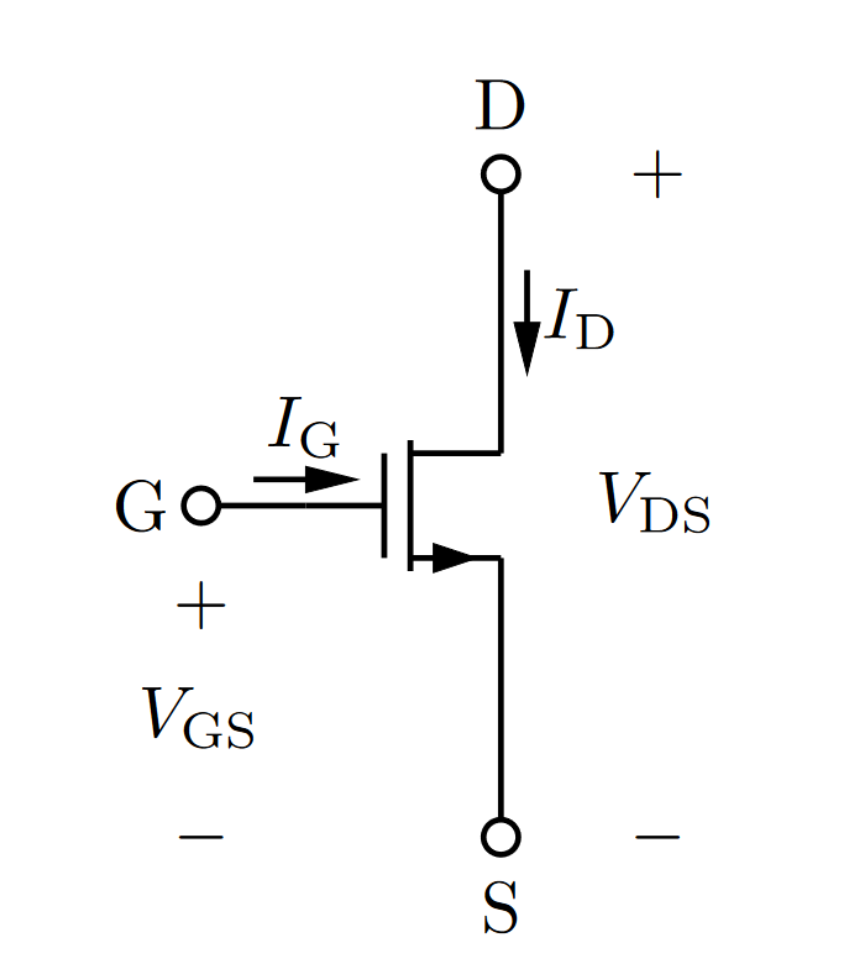
\includegraphics[width=6cm]{images/mosfet.png}
    \item Transistor equations: 
    \begin{align*}
        V_{DS} &= V_D -V_S\\
        V_{GS} &= V_G - V_S \\
        V_T &= V_G - V_D \\
        I_D &= \mu_n C_{ox} \left(\frac{W}{L}\right) \left[(V_{GS} - V_T)V_{DS} - \frac{1}{2} V_{DS}^2\right] \\
        &= k\left[(V_{GS} - V_T)V_{DS} - \frac{1}{2} V_{DS}^2\right], V_{DS} \leq V_{GS} - V_T, V_D \leq V_G - V_T \\
        I_D &= \mu_n C_{ox} \left(\frac{W}{L}\right) \left[\frac{1}{2} (V_{GS}-V_T)^2\right] \\
        &= k \left[\frac{1}{2} (V_{GS}-V_T)^2\right], V_{DS} \geq V_{GS} - V_T, V_D \geq V_G - V_T
    \end{align*}
    \item Condition for CSA distortion less than 10\%: $V_G < 0.2(V_G-V_T)$
    \item Gain of a CSA: $A = -R_Dk(V_G-V_T)=-g_m R_D$
\end{enumerate}
To find Thevenin voltage and Norton current:
\begin{itemize}
    \item[($R_{eq}$)] Turn off all independent sources (dependent
    sources remain unchanged) and calculate the resulting resistance at the
    desired port. Notice that you may have to apply the i-v test if resistors
    cannot be combined through series and parallel connections, or if the
    circuit includes dependent sources.
    \item[($V_{th}$)] Leave the desired port open-circuited
    (i.e. no load connected) and find the voltage across it.
    \item[($I_N$)] Short-circuit the desired port (i.e. connect
    a short circuit across the port) and find the current through it. 
\end{itemize}

\end{document}